% !chktex-file 8
% !chktex-file 1

% Document type
\documentclass[french,twoside]{article}
\usepackage{edify}

\usetikzlibrary{automata}
\usetikzlibrary{arrows}
\usetikzlibrary{positioning}

\title{Complexité en état d'opération sur des langages rationnels}
\date{\today}
\author{
  Edouard
  % LTeX: enabled=false
  HADDAG
  % LTeX: enabled=true
}
% LTeX: enabled=false
\logo{logo-univ-rouen-normandie-noir.png}
% LTeX: enabled=true
\headerrf{Université de Rouen Normandie}
\headerrs{Application Informatique}
\abs{
  Dans cet article, nous étudions deux transformations particulières de
  langages rationnels~: le << trognon >> et le << langage permuté >>. Nous
  définissons formellement ces deux constructions et proposons pour chacune un
  algorithme permettant de calculer un automate non déterministe reconnaissant
  le langage transformé. Nous démontrons la correction de ces algorithmes et
  analysons leur complexité en nombre d’états dans le pire des cas.
}

\begin{document}

\maketitle

\newpage

\tableofcontents

% !chktex-file 8

\section{Introduction}

\subsection{Prémisse}

\subsubsection{Langage}

\setframetitle{Langage}

\begin{frame}{\myframetitle}
  \begin{definition}[Langage]
    Un << langage >> \(L\) est un ensemble de mots sur un alphabet \(\Sigma\).
  \end{definition}

  \pause[]

  \begin{example}
    \vspace{-1.5\topsep}
    \begin{gather*}
      L = \{\varepsilon, aa, bb, abab\}
    \end{gather*}
  \end{example}

  \pause[]

  \begin{definition}[Le langage de l'ensemble des mots]
    L'ensemble des mots possible sur l'alphabet \(\Sigma\) sera noté
    \(\Sigma^*\).
  \end{definition}
\end{frame}

\subsubsection{Automate}

\setframetitle{Automate}

\begin{frame}{\myframetitle}
  \begin{definition}[Automate]
    \(M = (Q, I, F, \delta)\) avec \(Q = \{q_1, q_2, q_3\}\), \(I = \{q_1\}\)
    et \(F = \{q_3\}\).
    \begin{center}
      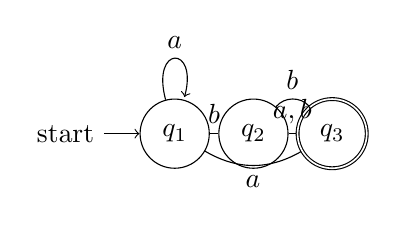
\begin{tikzpicture}
        \node[state, initial] (q1) {\(q_1\)};
        \node[state, right of=q1] (q2) {\(q_2\)};
        \node[state, accepting, right of=q2] (q3) {\(q_3\)};

        \draw
        (q1) edge[loop above] node{\(a\)} (q1)
        (q1) edge[above] node{\(b\)} (q2)
        (q1) edge[bend right, below] node{\(a\)} (q3)
        (q2) edge[above] node{\(a,b\)} (q3)
        (q3) edge[bend right=50, above] node{\(b\)} (q2);
      \end{tikzpicture}
    \end{center}
  \end{definition}
\end{frame}

\begin{frame}{\myframetitle}
  \begin{definition}[L'acceptation d'un mot]
    Le mot \(aba\) est << accepté >>~:
    \begin{center}
      \begin{tikzpicture}
        \node[state, initial] (q1) {\(q_1\)};
        \node[state, right of=q1] (q2) {\(q_2\)};
        \node[state, accepting, right of=q2] (q3) {\(q_3\)};

        \only<1> {\draw (q1) edge[loop above] node{\(a\)} (q1);}
        \only<1-2> {\draw (q1) edge[above] node{\(b\)} (q2);}
        \only<1-3> {\draw (q2) edge[above] node{\(a,b\)} (q3);}

        \only<2-> {\draw (q1) edge[loop above, red] node{\(a\)} (q1);}
        \only<3-> {\draw (q1) edge[above, red] node{\(b\)} (q2);}
        \only<4-> {\draw (q2) edge[above, red] node{\(a,b\)} (q3);}

        \draw
        (q3) edge[bend right=50, above] node{\(b\)} (q2)
        (q1) edge[bend right, below] node{\(a\)} (q3);
      \end{tikzpicture}
    \end{center}
  \end{definition}
\end{frame}

\begin{frame}{\myframetitle}
  \begin{definition}[Automate minimal]
    L'automate \(M_1\) est << minimal >> du langage \(L = \{ab\}\)~:

    \begin{minipage}{0.47\textwidth}
      \centering
      \begin{tikzpicture}[node distance=2.5cm]
        \node[state, initial] (0) {\(0\)};
        \node[state, right of=0] (1) {\(1\)};
        \node[state, accepting, below of=1] (2) {\(2\)};

        \node[above =.75cm of $(0)!0.5!(1)$, align=center] {\(M_1\)};

        \draw
        (0) edge[above] node{\(a\)} (1)
        (1) edge[right] node{\(b\)} (2);
      \end{tikzpicture}
    \end{minipage}
    \hfill
    \begin{minipage}{0.47\textwidth}
      \centering
      \begin{tikzpicture}[node distance=2.5cm]
        \node[state, initial] (0) {\(0\)};
        \node[state, right of=0] (1) {\(1\)};
        \node[state, accepting, below of=1] (2) {\(2\)};
        \node[state, left of=2] (3) {\(3\)};

        \node[above =.75cm of $(0)!0.5!(1)$, align=center] {\(M_2\)};

        \draw
        (0) edge[above] node{\(a\)} (1)
        (1) edge[right] node{\(b\)} (2)
        (0) edge[left] node{\(a\)} (3);
      \end{tikzpicture}
    \end{minipage}
  \end{definition}
\end{frame}

\subsubsection{Lien entre les langages et les automates}

\setframetitle{Lien entre les langages et les automates}

\begin{frame}{\myframetitle}
  \begin{definition}[Langage rationnel]
    Les langages << rationnels >> sont les langages reconnaissables par au
    moins un automate.
  \end{definition}
\end{frame}

\subsubsection{Complexité en état}

\setframetitle{Complexité en état}

\begin{frame}{\myframetitle}
  \begin{definition}
    La << complexité en état >> est une mesure d'un \textbf{langage}, elle est
    définie comme le nombre d'états de l'automate minimal du langage. Qui sera
    noté \(\mathcal{C}(L)\).
  \end{definition}
\end{frame}

\begin{frame}{\myframetitle}
  \begin{example}[%
      \only<1>{Définition d'une famille}%
      \only<2>{\(\mathcal{C}(A_2) = 2 + 2\)}%
    ]
    \centering
    \vspace{-1.5\topsep}
    \begin{gather*}
      A_n = \Sigma^* \cdot a \cdot \Sigma^n
    \end{gather*}
    \vspace{-2.25\topsep}

    \onslide<2-> {
      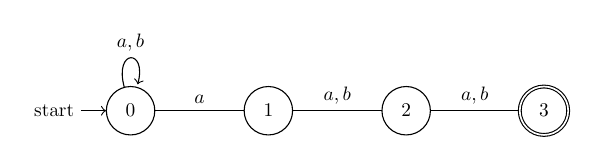
\begin{tikzpicture}[node distance=2.5cm, scale=0.7,transform shape]
        \node[state, initial] (0') {\(0\)};
        \node[state, right of=0'] (1') {\(1\)};
        \node[state, right of=1'] (2') {\(2\)};
        \node[state, accepting, right of=2'] (3') {\(3\)};

        \draw
        (0') edge[above] node{\(a\)} (1')
        (1') edge[above] node{\(a,b\)} (2')
        (2') edge[above] node{\(a,b\)} (3')
        (0') edge[loop above] node{\(a,b\)} (0');
      \end{tikzpicture}
    }
  \end{example}
\end{frame}

\begin{frame}{\myframetitle}
  \begin{definition}[Complexité en état opérationniel]
    La fonction \(f\) à une complexité \(g(n)\) si~:
    \begin{center}
      \begin{tikzpicture}[transform shape, scale=0.8]
        \node[draw, ellipse, minimum width=1.5cm] (A) at (-3,0) {\(A\)};
        \node[draw, rectangle, minimum width=2cm, minimum height=1cm]
        (F) at (0,0) {\(f\)};
        \node[draw, ellipse, minimum width=1.5cm] (C) at (3,0) {\(C\)};

        \node[left =0.25cm of A] {\(n\)};
        \node[right =0.25cm of C] {\(k \leq g(n)\)};

        \draw (A) -- (F);
        \draw (F) -- (C);
      \end{tikzpicture}
    \end{center}
  \end{definition}
\end{frame}

\section{Préliminaires}

Dans cette section préliminaire, nous allons rappeler les notions
fondamentales nécessaires à la compréhension du reste du document. Nous y
définirons notamment les concepts d’alphabet, de mot, de langage, d’automate
et de complexité en nombre d’états. Ces définitions seront accompagnées
d’exemples et de remarques pour en faciliter l’assimilation

% ----------------------------------------------------------------------------
\subsection{Les mots}

\begin{definition}[Alphabet]
  Un \textit{alphabet} \(\Sigma\) est un ensemble fini non-vide de
  \textit{symboles}.
\end{definition}

\begin{definition}[Mot]
  Un \textit{mot} est une suite finie de symboles sur un alphabet \(\Sigma\).
  Le mot composé de zéro symbole est appelé mot vide et est noté 
  \(\varepsilon\). De plus, l'ensemble des mots sera noté \(\Sigma^*\)
\end{definition}

\begin{example}
  \vspace{-\baselineskip}
  \begin{align*}
    \Sigma &= \{a, b, c, d\}, \\
    w &= abbcdda.
  \end{align*}
\end{example}

\begin{definition}[Longueur d'un mot]
  On parlera de la \textit{longueur d'un mot} \(w\) noté \(\lvert w \rvert\)
  pour désigner le nombre de symboles qui le composent. 
\end{definition}

\begin{example}
  \vspace{-\baselineskip}
  \begin{align*}
    w &= abbcdda, \\
    \lvert w \rvert &= 7.
  \end{align*}
\end{example}

\begin{definition}[Concaténation de deux mots]
  On notera la \textit{concaténation} de deux mots \(u = a_0 \cdots a_n\) et 
  \(v = b_0 \cdots b_m\) par \(u \cdot v\). Qui est ainsi égal à \(u \cdot v =
  a_0 \cdots a_n b_0 \cdots b_m\). On notera que~:

  \vphantom{}

  \begin{itemize}
    \item[\bullet] La concaténation est associative \((w \cdot u) \cdot v = w
      \cdot (u \cdot v)\).
    \item[\bullet] La concaténation admet un élément neutre \(u \cdot 
      \varepsilon = \varepsilon \cdot u = u\).
  \end{itemize}
\end{definition}

\begin{example}
  \vspace{-\baselineskip}
  \begin{align*}
    u &= aba, \\
    v &= cdcd, \\
    u \cdot v &= abacdcd.
  \end{align*}
\end{example}

\begin{definition}[Facteur, préfixe, suffixe d'un mot]
  Un \textit{facteur} \(u\) d'un mot \(w\) est une suite extraite de la suite
  de lettre qui composent le mot \(w\)~:
  \begin{align*}
    u \text{ est un facteur de } w \Longleftrightarrow \exists (v, x) \in
    (\Sigma ^ *)^2 ~|~ w = v \cdot u \cdot x.
  \end{align*} 

  \begin{itemize}
    \item[\bullet] Par ailleurs, on parlera de \textit{préfixe} quand \(v = 
      \varepsilon\).
    \item[\bullet] Enfin, on parlera de \textit{suffixe} quand \(x =
      \varepsilon\).
  \end{itemize}

  \vphantom{}

  Par ailleurs, on remarquera que \(\varepsilon\) est~: \textit{préfixe}, 
  \textit{suffixe} et \textit{facteur} de tout mot.
\end{definition}

\begin{example}
  Dans cet exemple, on a que \(u\) est un facteur de \(w\), que \(v\) est un
  préfixe de \(w\) et enfin que \(y\) est un suffixe de \(w\)~:
  \begin{align*}
    w &= abbcdda, \\
    u &= bcd, \\
    v &= abb, \\
    y &= dda.
  \end{align*}
\end{example}

\begin{definition}[Le miroir d'un mot]
  Le \textit{miroir} d'un mot \(w\) noté \(\overleftarrow{w}\). Qui est ainsi
  défini récursivement comme ceci~:
  \begin{align*}
    \overleftarrow{\varepsilon} &= \varepsilon, \\
    \overleftarrow{u \cdot a} &= a \cdot \overleftarrow{u}, \\
    \text{Avec } a \in~&\Sigma \text{ et } u \in \Sigma^*.
  \end{align*}
\end{definition}

\begin{example}
  \vspace{-\baselineskip}
  \begin{align*}
    w &= abbcdda, \\
    \overleftarrow{w} &= addcbba.
  \end{align*}
\end{example}

% ----------------------------------------------------------------------------
\subsection{Les langages}

\begin{definition}[Langage]
  Un \textit{langage} \(L\) est un ensemble de mots sur un alphabet fini
  \(\Sigma\). On appellera \textit{langage vide} le langage ne comportant
  aucun mot et sera noté \(\varnothing\).
\end{definition}

\begin{example}
  \vspace{-\baselineskip}
  \begin{align*}
    \Sigma &= \{a, b, c, d\}, \\
    L_1 &= \{a, aa, bc, da, \varepsilon\}, \\
    L_2 &= \varnothing.
  \end{align*}
\end{example}

\begin{definition}[L'union de langages]
  L'\textit{union} de deux langages sera notée \(L_1 \cup L_2\) et est définie
  comme ceci~:
  \begin{gather*}
      L_1 \cup L_2 = \{w \in \Sigma ^ * \mid w \in L_1 \lor w \in L_2\}.
  \end{gather*}
\end{definition}

\begin{example}
  \vspace{-\baselineskip}
  \begin{align*}
    L_1 &= \{\varepsilon, a, aa, bc, da\}, \\
    L_2 &= \{d, aa, cd\}, \\
    L_1 \cup L_2 &= \{\varepsilon, a, d, aa, cd, bc, da\}. \\
  \end{align*}
\end{example}

\begin{definition}[Concaténation de langages]
  La \textit{concaténation} de deux langages sera notée \(L_1 \cdot L_2\) et
  est définie grâce à la concaténation des mots qui composent les langages~:
  \begin{gather*}
    L_1 \cdot L_2 = \{u \cdot v ~|~ u \in L_1, v \in L_2\}.
  \end{gather*}
\end{definition}

\begin{example}
  \vspace{-\baselineskip}
  \begin{align*}
    L_1 &= \{\varepsilon, a, aa\}, \\
    L_2 &= \{d, cc\}, \\
    L_1 \cdot L_2 &= \{d, ad, aad, cc, acc, aacc\}.
  \end{align*}
\end{example}

\begin{definition}[Copie n-ième d'un langage]
  La \textit{copie n-ième} d'un langage \(L\) notée \(L^n\) et est définie
  récursivement comme ceci~:
  \begin{align*}
    L^0 &= \{\varepsilon\}, \\
    L^n &= L^{n - 1} \cdot L.
  \end{align*}
\end{definition}

\begin{example}
  \vspace{-\baselineskip}
  \begin{align*}
    L &= \{\varepsilon, a\}, \\
    L^3 &= \{\varepsilon, a, aa, aaa\}.
  \end{align*}
\end{example}

\begin{definition}[L'étoile (de \textsc{Kleene}) d'un langage]
  L'\textit{étoile} (de \textsc{Kleene}) d'un langage noté \(L^*\), sera
  définie comme ceci~:
  \begin{gather*}
    L^* = \bigcup_{i \geq 0} L^i.
  \end{gather*}
\end{definition}

\begin{example}
  \vspace{-\baselineskip}
  \begin{align*}
    L &= \{a\}, \\
    L^* &= \{\varepsilon\} \cup \{a\} \cup \{aa\} \cup \cdots
  \end{align*}
\end{example}

\begin{remark}
  Grâce à cette opération, on comprend dorénavant la notion \(\Sigma^*\) comme
  l'ensemble des mots de l'alphabet \(\Sigma\), il pourra donc aussi être vu
  comme le langage contenant tous les mots.
\end{remark}

\begin{definition}[Langages rationnel]
  On note \(Rat(\Sigma^*)\) le plus petit ensemble de langages sur
  \(\Sigma^*\) vérifiant les propriétés suivantes~:

  \vphantom{}

  \begin{itemize}
    \item[\bullet] \(\varnothing \in Rat(\Sigma^*)\).
    \item[\bullet] \(\{a\} \in Rat(\Sigma^*) \text{ avec } a \in \Sigma\).
    \item[\bullet] \(Rat(\Sigma^*)\) est fermé pour les opérations d'union,
    de concaténation et pour l'étoile.
  \end{itemize}
\end{definition}

\begin{remark}
  Pour simplifier l’écriture, nous écrirons \(+\) pour représenter l’union, et
  nous utiliserons également \(ab\) au lieu de \(\{ab\}\).
\end{remark}

\begin{example}
  \vspace{-\baselineskip}
  \begin{align*}
    L = \varnothing + (a^* \cdot (b + \varepsilon)).
  \end{align*}
\end{example}

% ----------------------------------------------------------------------------
\subsection{Les automates}

Nous allons parler des automates sans \(\varepsilon\)-transition (des 
automates utilisent des \\\(\varepsilon\)-transitions, comme ceux de 
\textsc{Thompson} \cite{thompson1968programming}, utilisés par nos 
ordinateurs). Pour autant, les automates que nous verrons ne sont pas limités
par le manque de ces transitions.

\begin{definition}[Automate]
  Un \textit{automate} est un objet mathématique \textit{reconnaissant} un
  langage. On notera \(M \in AFN(\Sigma, \eta)\) l'automate qui a pour
  \textit{transition} des valeurs dans \(\Sigma\), des valeurs d'\textit{état}
  dans \(\eta\).

  \vphantom{}

  On aura aussi, \(AFN(\Sigma, \eta)\), l'ensemble des automates finis 
  \textit{non déterministes} de valeur de transition dans \(\Sigma\) et de 
  valeur d'état dans \(\eta\). Enfin, on écrira \(L(M)\) pour désigner le
  langage qu'il reconnait.

  \vphantom{}

  Un automate est un tuple qu'on peut écrire de cette forme \(M = (Q, I, F, 
  \delta)\) avec~:
  \begin{alignat*}{3}
    &\cmath{Q} && \subseteq \eta &&\text{États de l'automate.} \\
    &\cmath{I} && \subseteq Q &&\text{États initiaux.} \\
    &\cmath{F} && \subseteq Q &&\text{États finaux.} \\
    &\cmath{\delta}&&: Q \times \Sigma \to \mathcal{P}(Q)~ &&\text{Fonction de
    transition.}
  \end{alignat*}
\end{definition}

\begin{remark}[Extension de la fonction de transition]
  On peut étendre la fonction de transition pour ce qu’elle prenne en entrée
  non plus un simple symbole, mais un mot. Sa signature devient alors 
  \(\delta~: Q \times \Sigma^* \to \mathcal{P}(Q)\), et elle est définie comme
  suit~:
  \begin{align*}
    \delta(q, \varepsilon) &= \{q\}, \\
    \delta(q, a \cdot w) &= \bigcup_{p \in \delta(q, a)} \delta(p, w),
    \text{ avec } a \in \Sigma.
  \end{align*}
\end{remark}

\begin{definition}[Reconnaissance d'un mot par un automate]
  Un mot est \textit{reconnu} (ou \textit{accepté}) s'il existe une suite de
  transition partant d'un état initial vers un état final~:
  \begin{align*}
    w \text{ est accepté par } M \Longleftrightarrow \left( \bigcup_{i \in I}
    \delta(i, w) \right) \cap F \neq \varnothing.
  \end{align*}
\end{definition}

\begin{definition}[Langage d'un automate]
  Le \textit{langage d'un automate} est donc l'ensemble des mots qu'il
  reconnait~:
  \begin{align*}
    L(M) = \{w \in \Sigma^* \mid w \text{ est accepté par } M\}.
  \end{align*}
\end{definition}

\begin{example}[Représentation d'un automate]
  Un automate peut se représenter à l'aide d'un graphe orienté et valué
  particulier. Par exemple, si on veut représenter \(M = (\{q_1, q_2, q_3,
  q_4, q_5\}, \{q_1, q_2\},\{q_2, q_3\}, \delta)\) avec \(M \in AFN(\Sigma,
  \eta)\), \(\Sigma = \{a, b\}\), \(\eta = \{q_1, q_2, q_3, q_4, q_5\}\) et
  \(\delta\) défini comme ceci~:
  \begin{align*}
    \delta(q_1, a) &= \{q_2, q_4\}, & \delta(q_3, b) & = \{q_4\}, \\
    \delta(q_1, b) &= \varnothing,  & \delta(q_4, a) & = \{q_5\}, \\
    \delta(q_2, a) &= \varnothing,  & \delta(q_4, b) & = \{q_3\}, \\
    \delta(q_2, b) &= \varnothing,  & \delta(q_5, a) & = \{q_4\}, \\
    \delta(q_3, a) &= \{q_3\},      & \delta(q_5, b) & = \{q_5\}.
  \end{align*}
  \begin{figure}[H]
    \centering
    \captionsetup{type=figure,justification=centering}
    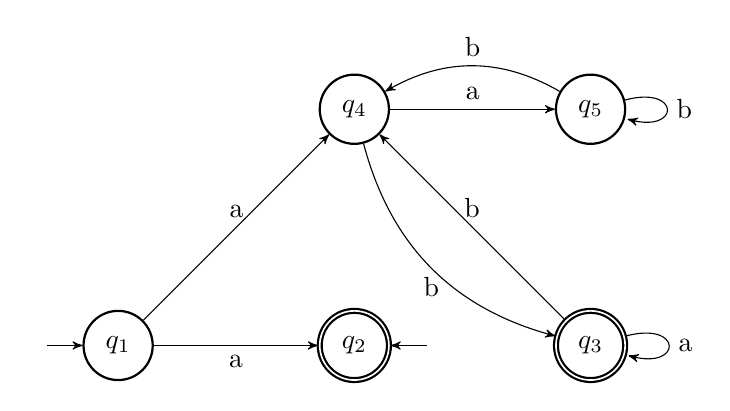
\begin{tikzpicture}
      \tikzset{
        ->,
        >=stealth',
        node distance=3cm,
        every state/.style={thick},
        initial text=$ $,
      }
      \node[state, initial] (q1) {\(q_1\)};
      \node[state, initial right, accepting, right of=q1] (q2) {\(q_2\)};
      \node[state, above of=q2] (q4) {\(q_4\)};
      \node[state, accepting, right of=q2] (q3) {\(q_3\)};
      \node[state, right of=q4] (q5) {\(q_5\)};

      \draw
        (q1) edge[above] node{a} (q4)
        (q1) edge[below] node{a} (q2)
        (q4) edge[bend right, below] node{b} (q3)
        (q4) edge[above] node{a} (q5)
        (q3) edge[above] node{b} (q4)
        (q3) edge[loop right] node{a} (q3)
        (q5) edge[bend right, above] node{b} (q4)
        (q5) edge[loop right] node{b} (q5);
    \end{tikzpicture}
    \caption{Exemple de représentation graphique d'un automate.}
  \end{figure}

  On peut voir que les états initiaux ont une petite flèche qui pointe sur eux
  et que les états finaux ont un double contour. Et, que les transitions sont
  symbolisées par des flèches entre les états et que ces flèches sont 
  labellisées.
\end{example}

\begin{definition}[Automate déterministe]
  Un automate est dit \textit{déterministe} quand tous ses états vont au
  maximum à un état par symbole et que l'automate ne possède qu'un seul état
  initial.
  \begin{gather*}
    \lvert I \rvert = 1 \land \forall q \in Q, \forall a \in \Sigma, \lvert 
    \delta(q, a) \rvert \leq 1 \Longleftrightarrow M \in DFA(\Sigma, \eta)
  \end{gather*}
  avec \(DFA(\Sigma, \eta)\) l'ensemble des automates déterministe.
\end{definition}

\begin{example}[Représentation d'un automate déterministe]
  \vspace{-\baselineskip}
  \begin{figure}[H]
    \centering
    \captionsetup{type=figure,justification=centering}
    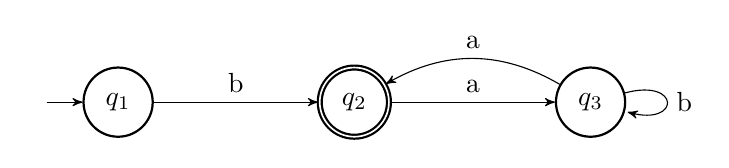
\begin{tikzpicture}
      \tikzset{
        ->,
        >=stealth',
        node distance=3cm,
        every state/.style={thick},
        initial text=$ $,
      }
      \node[state, initial] (q1) {\(q_1\)};
      \node[state, accepting, right of=q1] (q2) {\(q_2\)};
      \node[state, right of=q2] (q3) {\(q_3\)};

      \draw
        (q1) edge[above] node{b} (q2)
        (q2) edge[above] node{a} (q3)
        (q3) edge[bend right, above] node{a} (q2)
        (q3) edge[loop right] node{b} (q3);
    \end{tikzpicture}
    \caption{Exemple de représentation graphique d'un automate déterministe.}
  \end{figure}
\end{example}

\begin{definition}[L'ensemble des langages reconnaissable]
  On note \(Rec(\Sigma^*)\), l'ensemble des langages de \(\Sigma^*\) dit 
  \textit{reconnaissable}~:
  \begin{align*}
    L \in Rec(\Sigma^*) \Longleftrightarrow \exists M \in NFA(\Sigma, \eta)
    \land L = L(M).
  \end{align*}
\end{definition}

\begin{theorem}[Théorème de \textsc{Kleene}]
  Le mathématicien \textsc{Stephen Cole Kleene} a démontré que~:
  \begin{align*}
    Rec(\Sigma^*) = Rat(\Sigma^*).
  \end{align*}
  On pourra alors passer de langage rationnel à automate et vice-versa.
\end{theorem}

\begin{remark}
  La notation \(\lvert M \rvert\) représentera le nombre d'états de l'automate
  \(M\).
\end{remark}

\begin{definition}[Automate minimal]
  Un automate est dit \textit{minimal} lorsqu’il s’agit de l’automate ayant le
  plus petit nombre d’états possible qui reconnaît un langage donné~:
  \begin{align*}
    M \text{ est minimal} \Longrightarrow \nexists N \in NFA(\Sigma, \eta)
    \land L(M) = L(N).
  \end{align*}
  On parlera d'automate \text{déterministe minimal} quand~:
    \begin{align*}
    M \text{ est déterministe minimal} \Longrightarrow \nexists N \in 
    DFA(\Sigma, \eta) \land L(M) = L(N).
  \end{align*}
\end{definition}

\begin{example}[Représentation d'un automate minimal]
  Dans cet exemple, l'automate \(M_2\) est bien plus petit que l'automate
  \(M_1\), c'est même le plus petit automate reconnaissant leur langage
  (\(a^*\))
  \begin{figure}[H]
    \centering
    \captionsetup{type=figure,justification=centering}
    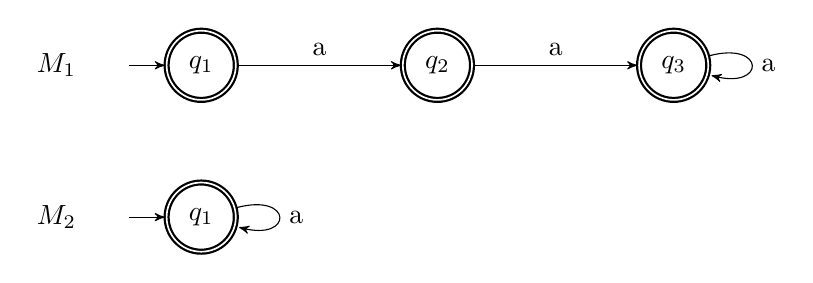
\begin{tikzpicture}
      \tikzset{
        ->,
        >=stealth',
        node distance=3cm,
        every state/.style={thick},
        initial text=$ $,
      }
      \node[state, initial, accepting] (q1) {\(q_1\)};
      \node[left=1cm of q1] {\(M_1\)};
      \node[state, accepting, right of=q1] (q2) {\(q_2\)};
      \node[state, accepting, right of=q2] (q3) {\(q_3\)};
      \node[state, initial, accepting, below=1cm of q1] (q4) {\(q_1\)};
      \node[left=1cm of q4] {\(M_2\)};

      \draw
        (q1) edge[above] node{a} (q2)
        (q2) edge[above] node{a} (q3)
        (q3) edge[loop right] node{a} (q3)
        (q4) edge[loop right] node{a} (q4);
    \end{tikzpicture}
    \caption{
      Exemple de représentation graphique d'un automate minimal.
    }\label{fig:ex_minimal}
  \end{figure}
\end{example}

%-----------------------------------------------------------------------------
\subsection{La complexité en état}

\begin{definition}[Complexité en état d'un langage (rationnel)]
  La \textit{complexité en état} d'un langage est le nombre d'états de
  l'automate minimal reconnaissant ce langage~:
  \begin{gather*}
    \mathcal{C}(L) = \lvert M \rvert \land L(M) = L \text{ avec} \\ 
    M \text{ est un automate minimal.}
  \end{gather*}
  Cette complexité se scinde en deux parties~:

  \vphantom{}

  \begin{itemize}
    \item[\bullet] La complexité non déterministe (\(\mathcal{C}_{ndet}\))
    quand~:
    \begin{align*}
      M \in NFA(\Sigma, \eta).
    \end{align*}
    \item[\bullet] La complexité déterministe (\(\mathcal{C}_{det}\))
    lorsque~:
    \begin{align*}
      M \in DFA(\Sigma, \eta).
    \end{align*}
  \end{itemize}
\end{definition}

\begin{example}
  Si on reprend le langage de la figure~\ref{fig:ex_minimal}, \(M_2\) est
  l'automate minimal reconnaissant \(a^*\) et il n'a qu'un état, de ce fait ce
  langage à une complexité en état déterministe de \(1\). Et, donc aussi, une
  complexité non déterministe de \(1\), puisque tout automate déterministe est
  dans \(NFA(\Sigma, \eta)\) et qu'on ne peut pas faire un automate à moins
  d'un état.
\end{example}

\begin{definition}[Complexité en état opérationnel]
  La \textit{complexité en état opérationnel} peut être vu comme la borne
  supérieure de la complexité en état du langage produit par l'opération.
  Autrement dit, \(f\) a une complexité de \(g(n_1, \ldots, n_k)\) quand~:
  \begin{align*}
    \forall (L_1, \ldots, L_k) \in \mathcal{P}(\Sigma^*) \quad
    \mathcal{C}(f(L_1, \ldots, L_k)) \leq 
    g(\mathcal{C}(L_1), \ldots, \mathcal{C}(L_k)).
  \end{align*}
  De même que la complexité en état, la complexité en état opérationnel se
  scinde en deux parties~:

  \vphantom{}

  \begin{itemize}
    \item[\bullet] La complexité non déterministe quand~:
    \begin{align*}
      \mathcal{C}_{ndet}(f(L_1, \ldots, L_k)) \leq 
      g(\mathcal{C}_{ndet}(L_1), \ldots, \mathcal{C}_{ndet}(L_k)).
    \end{align*}
    \item[\bullet] La complexité déterministe lorsque~:
    \begin{align*}
      \mathcal{C}_{det}(f(L_1, \ldots, L_k)) \leq 
      g(\mathcal{C}_{det}(L_1), \ldots, \mathcal{C}_{det}(L_k)).
    \end{align*}
  \end{itemize}
\end{definition}

\begin{remark}
  La complexité en état déterministe sera toujours supérieure ou égale à la
  complexité en état non déterministe, dû au fait que les automates
  déterministes sont aussi des automates non déterministe, mais avec des
  contraintes en plus.
\end{remark}

\begin{example}
  Voici quelques complexités en état opérationnel connues et importantes~:
  \begin{table}[H]
    \centering
    \captionsetup{type=table,justification=centering}
    \renewcommand{\arraystretch}{2}
    \begin{tabular}{|c|c|c|}
    \hline
      \textbf{Fonction} & \textbf{Complexité} & \textbf{Source} \\
      \hline
      L'union non déterministe & \(m + n\) & \textsc{Holzer} et 
      \textsc{Kutrib}~\cite{holzer_kutrib} \\
      \hline
      L'union déterministe & \(m n\) & 
      \textsc{Maslov}~\cite{maslov1970estimates} \\
      \hline
      L'intersection non déterministe & \(m n\) & \textsc{Holzer} et 
      \textsc{Kutrib}~\cite{holzer_kutrib} \\
      \hline
      L'intersection déterministe & \(m n\) & 
      \textsc{Maslov}~\cite{maslov1970estimates} \\
      \hline
      La concaténation non déterministe & \(m + n\) & \textsc{Holzer} et 
      \textsc{Kutrib}~\cite{holzer_kutrib} \\
      \hline
      La concaténation déterministe & \(m 2^n - 2^{n - 1}\) & 
      \textsc{Maslov}~\cite{maslov1970estimates} \\
      \hline
      L'étoile (de \textsc{Kleene}) non déterministe & \(n + 1\) &
      \textsc{Holzer} et \textsc{Kutrib}~\cite{holzer_kutrib} \\
      \hline
      L'étoile (de \textsc{Kleene}) déterministe & \(\frac{3}{4}2^n\) & 
      \textsc{Maslov}~\cite{maslov1970estimates} \\
      \hline
    \end{tabular}
    \caption{
      Tableau de complexité en état opérationnel de plusieurs opérations.
    }
  \end{table}
\end{example}

\begin{remark}[Complexité de la déterminisation]
  L'opération de \textit{déterminisation}, c'est-à-dire l'opération de rendre
  un automate non déterministe quelconque en un automate déterministe à une
  complexité en état de \(2^n\).

  Même si cette opération ne rentre pas réellement dans notre définition de la
  complexité en état, car prenant en entrée un automate non déterministe et
  renvoyant un automate déterministe.
\end{remark}

\section{Le trognon d'un langage}

Dans cette partie, nous nous concentrerons sur un langage bien particulier, le
<< trognon >>. Dans un premier temps, nous définirons formellement ce langage.
Enfin, nous présenterons un algorithme de << grignotage >> permettant de le
calculer à partir d'un automate non déterministe, l'automate du trognon du
langage de l'automate initial. Nous présenterons ensuite une preuve de cet
algorithme ainsi que la complexité dans le pire des cas de celui-ci. Enfin,
pour finir, nous conclurons cette partie en faisant une courte synthèse de ce
qu'on aura vu et de la possible continuation.

\subsection{Définition}

\begin{definition}[Le langage trognon]
  Le langage \(Core(L)\) (aussi noté \(Trognon(L)\)) est construit à partir de
  \(L\) en retirant, pour chaque mot de \(L\), un préfixe dont le miroir est
  également un suffixe~; ce suffixe est, lui aussi, retiré~:
  \begin{align*}
    Core(w) &= \{v \in \Sigma^* \mid \exists u \in \Sigma^* \land w = u \cdot v
    \cdot \overleftarrow{u}\}, \\
    Core(L) &= \bigcup_{w \in L} Core(w).
  \end{align*}
\end{definition}

\begin{example}
  \vspace{-\baselineskip}
  \begin{align*}
    L &= \{a, b, aa, aabcaa\}, \\
    Core(L) &= \{\varepsilon, a, b, bc, abca, aabcaa\}.
  \end{align*}
\end{example}

Maintenant que nous savons ce qu’est le trognon d’un langage, nous allons
présenter un algorithme permettant de construire un automate le reconnaissant,
à partir d’un automate reconnaissant le langage initial.

\subsection{Algorithme de grignotage}

Notre algorithme prendra en entrée un automate non déterministe et renverra un
automate non déterministe. Mais, avant de rentrer dans le dur de l'algorithme,
nous regardons le principe de l'algorithme, puis nous verrons sa définition
formelle.

\subsubsection{Principe de l'algorithme}

Le principe de cet algorithme est assez simple, si on prend l'automate 
suivant~:
\begin{figure}[H]
  \centering
  \captionsetup{type=figure,justification=centering}
  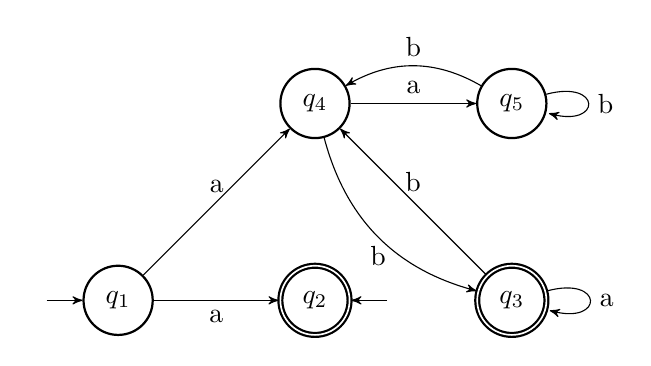
\begin{tikzpicture}
    \tikzset{
      ->,
      >=stealth',
      node distance=2.5cm,
      every state/.style={thick},
      initial text=$ $,
    }
    \node[state, initial] (q1) {\(q_1\)};
    \node[state, initial right, accepting, right of=q1] (q2) {\(q_2\)};
    \node[state, above of=q2] (q4) {\(q_4\)};
    \node[state, accepting, right of=q2] (q3) {\(q_3\)};
    \node[state, right of=q4] (q5) {\(q_5\)};

    \draw
      (q1) edge[above] node{a} (q4)
      (q1) edge[below] node{a} (q2)
      (q4) edge[bend right, below] node{b} (q3)
      (q4) edge[above] node{a} (q5)
      (q3) edge[above] node{b} (q4)
      (q3) edge[loop right] node{a} (q3)
      (q5) edge[bend right, above] node{b} (q4)
      (q5) edge[loop right] node{b} (q5);
  \end{tikzpicture}
  \caption{Exemple d'un automate avant grignotage.}
\end{figure}

Nous devons alors le << grignoté >> de tous les mots pour en faire l'automate
reconnaissant le trognon du langage. Avant d'essayer de le grignoter de tous
les mots, on va tenter de le grignoter d'un seul mot, \(ab\). On va donc
simplement << avancer >> les états initiaux de la transition \(ab\) et 
<< reculer >> les états finaux de la transition \(ab\)~:
\begin{align*}
  I' &= \bigcup_{i \in I} \delta(i, ab) = \{q_3\}, \\
  F' &= \bigcup_{f \in F} \delta^{-1}(f, ab) = \{q_4\}.
\end{align*}
avec \(\forall p \in \delta^{-1}(q, w) \Longrightarrow q \in
\delta(p, w)\).

\vphantom{}

Et, le reste de l'automate ne changerait pas, ce qui nous donnerait à la fin~:
\begin{figure}[H]
  \centering
  \captionsetup{type=figure,justification=centering}
  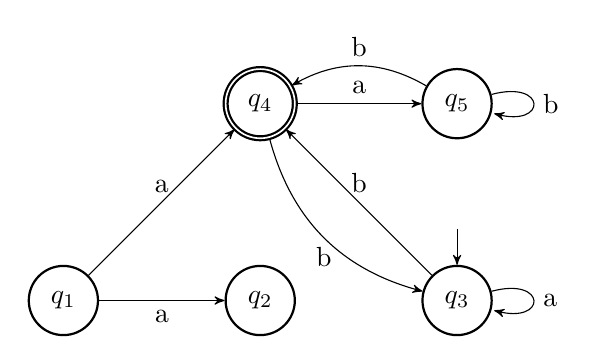
\begin{tikzpicture}
    \tikzset{
      ->,
      >=stealth',
      node distance=2.5cm,
      every state/.style={thick},
      initial text=$ $,
    }
    \node[state] (q1) {\(q_1\)};
    \node[state, right of=q1] (q2) {\(q_2\)};
    \node[state, accepting, above of=q2] (q4) {\(q_4\)};
    \node[state, initial above, right of=q2] (q3) {\(q_3\)};
    \node[state, right of=q4] (q5) {\(q_5\)};

    \draw
      (q1) edge[above] node{a} (q4)
      (q1) edge[below] node{a} (q2)
      (q4) edge[bend right, below] node{b} (q3)
      (q4) edge[above] node{a} (q5)
      (q3) edge[above] node{b} (q4)
      (q3) edge[loop right] node{a} (q3)
      (q5) edge[bend right, above] node{b} (q4)
      (q5) edge[loop right] node{b} (q5);
  \end{tikzpicture}
  \caption{Exemple d'un automate après grignotage de \(ab\).}
\end{figure}

\begin{definition}[Grignotage d'un automate par un mot]
  Soit \(M = (Q, I, F, \delta)\), un automate, le \emph{grignotage} de \(M\)
  par un mot \(w\) sera l'automate~:
  \begin{gather*}
    Nibbling(M, w) = (Q, I', F', \delta), \\
    I' = \bigcup_{i \in I} \delta(i, w) \land F' = \bigcup_{f \in F}
    \delta^{-1}(f, w). \\
  \end{gather*}
\end{definition}

\begin{lemma}[Premier lemme du grignotage]\label{lemma:grignotage}
  Si un mot \(w\) est reconnu par \(Nibbling(M, v)\), alors \(v \cdot w \cdot
  \overleftarrow{w}\) est reconnu par M.
  \begin{align*}
    \forall M \in NFA(\Sigma, \eta) \land \forall v \in \Sigma^* 
    \land N = Nibbling(M, v) \land w \in L(N) \Longleftrightarrow v \cdot w
    \cdot \overleftarrow{v} \in L(M).
  \end{align*}
\end{lemma}

\begin{lemma}[Second lemme du grignotage]\label{lemma:grignotage2}
  Soit un automate \(M \in NFA(\Sigma, \eta)\), et un mot \(w = u \cdot v
  \cdot \overleftarrow{u} \in L(M)\), si~:
  \begin{align*}
  \exists (x, y, z) \in (\Sigma^*)^3 \colon Nibbling(M, y) = Nibbling(M, x)
  \land u = x \cdot z \Longrightarrow (y \cdot z) \cdot v \cdot
  \overleftarrow{(y \cdot z)} \in L(M).
  \end{align*}
\end{lemma}

Il nous reste donc à présent à calculer le grignoté de tous les mots dits
<< pertinents >>, puis à effectuer l'union non déterministe des automates
ainsi obtenus.

\vphantom{}

Cependant, une question importante demeure~: quels sont les mots que l’on
qualifie de pertinents~?

\vphantom{}

Une première intuition serait de considérer tous les fragments internes des
mots du langage, autrement dit toutes les sous-parties situées entre le début
et la fin, ce que l’on pourrait appeler, de manière imagée, \textit{la chair}
du mot (par opposition au trognon).

\vphantom{}

Mais, cette approche soulève un problème~: le langage étant, en général,
infini, il existe potentiellement une infinité de << chairs >>. Une telle
démarche, si elle n’est pas restreinte, est alors incalculable en pratique.

\begin{definition}[La chair d'un langage]
  Le langage \(Flesh(L)\) (aussi noté \(Chair(L)\)) est construit à partir de
  \(L\) en gardant, pour chaque mot de \(L\), un préfixe dont le miroir est
  également un suffixe~:
  \begin{align*}
    Flesh(w) &= \{u \in \Sigma^* \mid \exists v \in \Sigma^* \land w = u
    \cdot v \cdot \overleftarrow{u}\}, \\
    Flesh(L) &= \bigcup_{w \in L} Flesh(w).
  \end{align*}
\end{definition}

\begin{example}
  \vspace{-\baselineskip}
  \begin{align*}
    L &= \{a, b, aa, aabcaa\}, \\
    Flesh(L) &= \{\varepsilon, a, b, aa\}.
  \end{align*}
\end{example}

Puisque l’automate reconnaissant le langage de départ est fini, notons \(n\)
son nombre d’états. Si un mot \(u\) appartient à la chair d’un mot, et que sa
longueur vérifie \(\lvert u \rvert \geq n\), alors la lecture de \(u\) force
la réapparition d’au moins un état (par le \textit{principe des tiroirs}). Il
en résulte l’existence d’un cycle dans l'automate de départ.

\vphantom{}

L’algorithme explore donc tous les mots \(w \in \Sigma^*\) en construisant
successivement les automates grignotés \(N = Nibbling(M, w)\). Puisque le
nombre d’automates à états fixes est fini, on aboutit forcément à une
répétition~: il existe un mot plus court \(u\) tel que
\begin{align*}
N = Nibbling(M, u) \land \lvert u \rvert < \lvert w \rvert.
\end{align*}

À partir de ce moment, il n’est plus nécessaire << d’étendre >> \(w\), car
tout mot préfixé par \(w\) aurait déjà été obtenu via un préfixe plus court.
Cette condition garantit l’arrêt de l’algorithme et garantit que l’on ne
construit qu’un nombre fini d’automates.

\subsubsection{Formalisation de l'algorithme}

Maintenant que nous avons l'idée de l'algorithme, nous verrons sa
définition formelle~:
\begin{minted}{text}
nibbling(M):
  N |\leftarrow| M
  la |\leftarrow \{\,\texttt{M}\,\}|
  lw |\leftarrow| queue_empty()
  enqueue(lw, |\varepsilon|)
  |\textbf{while}| lw |\!\(\neq \varnothing\)| |\textbf{do}|
    |\textbf{for}| s |\textbf{in}| |\Sigma| |\textbf{do}|
      w |\leftarrow| queue_dequeue(lw) |\!\cdot\!| s
      A |\leftarrow \(Nibbling(\,\texttt{M},\; \texttt{w}\,)\)|
      |\textbf{if}| A.I |\(\!\neq \varnothing\) \land| A.F |\(\!\neq \varnothing\) \land| A |\!\(\notin\)\!| la |\textbf{then}|
        N |\leftarrow| N |\cup| A
        la |\leftarrow \texttt{la} \cup \{\,\texttt{A}\,\}|
        enqueue(lw, w)
  |\textbf{return}| N
\end{minted}

\begin{remark}
  On observe que l’algorithme effectue un parcours en largeur de
  l’arborescence des mots. Cela garantit que tous les mots de longueur
  strictement inférieure ont été explorés avant de commencer à << grignoter >>
  ceux de longueur supérieure.
\end{remark}

\subsection{Preuve de notre algorithme}

Pour prouver que notre algorithme est correct et construit bien l'automate
du trognon d'un langage, nous allons d'abord montrer que tous mots reconnus
par l'automate sont des mots appartenant au trognon du langage. Enfin, nous
allons montrer que tous les mots du trognon d'un langage sont reconnu par
l'automate.

\subsubsection{Tous les mots reconnus sont des mots du trognon}

\begin{proof}
  Soit \(M \in NFA(\Sigma, \eta)\), \(N = \texttt{nibbling}(M)\) et un mot
  \(w\) reconnu par l'automate \(N\). S'il est reconnu par \(N\), c'est qu'il
  est reconnu par au moins un automate \(Nibbling(M, v)\) qui compose \(N\).
  Or, par le lemme~\ref{lemma:grignotage}, alors \(v \cdot w \cdot
  \overleftarrow{v}\) est reconnu par \(M\), et donc \(w\) fait partie de
  \(Core(L(M))\).
\end{proof}

\subsubsection{Tous les mots du trognon sont reconnus}

\begin{proof}
  Pour prouver que tous les mots du trognon de \(M \in NFA(\Sigma, \eta)\)
  sont bien reconnus par l'automate \(N = \texttt{nibbling}(M)\), nous allons
  faire une preuve par récurrence sur la longueur de la chair d'un mot \(w =
  u \cdot v \cdot \overleftarrow{u}\) du langage \(L(M)\)~:

  \vphantom{}

  \begin{itemize}
    \item[\bullet~\textbf{Initialisation~:}] \(\lvert u \rvert = 0\)

      Si \(\lvert u \rvert = 0 \Longleftrightarrow u = \varepsilon
      \Longleftrightarrow v = w\).

      \vphantom{}
      
      Ensuite, puisque nous faisons l'union de l'automate \(M\) dans notre
      algorithme~:
      \begin{align*}
        w \in L(M) \Longleftrightarrow v \in L(M) \Longleftrightarrow v \in
        L(\texttt{nibbling}(M)).
      \end{align*}

    \item[\bullet~\textbf{Hérédité~:}] \(\lvert u \rvert \geq 1\)
      \begin{itemize}
        \item[\circ] Si \(Nibbling(M, u)\) fait partie des automates dont on a
          fait l'union dans notre algorithme, alors par le
          lemme~\ref{lemma:grignotage}~:
          \begin{align*}
              v \in L(Nibbling(M, u)) \Longleftrightarrow v \in
              L(\texttt{nibbling}(M)).
          \end{align*}

        \item[\circ] Sinon cela veut dire que~:
          \begin{align*}
            \exists (y, x, z) \in \Sigma^* \colon Nibbling(M, y) = 
            Nibbling(M, x) \land u = x \cdot z \land \lvert y \rvert < \lvert x 
            \rvert.
          \end{align*}
          On s'intéresse donc au mot \(w' =  (y \cdot z) \cdot v \cdot
          \overleftarrow{(y \cdot z)}\) qui est dans \(L(M)\) par le
          lemme~\ref{lemma:grignotage2}, or par hypothèse de récurrence
          (\(\lvert y \cdot z \rvert < \lvert u \rvert\)) \(v \in
          L(\texttt{nibbling}(M))\).
      \end{itemize}
  \end{itemize}
\end{proof}

\newpage
\subsection{Pire cas de notre algorithme}

Dans cette section, nous établirons une borne supérieure sur le nombre
d’états de l’automate que notre algorithme peut engendrer. Cette estimation,
distincte de la complexité du trognon d’un langage, nous offre néanmoins un
plafond pour la complexité en états.

\vphantom{}

Dans notre pire cas, notre algorithme fera l'union de tous les automates
distincts qu'ont les mêmes états et la même fonction de transition. La seule
chose qui peut changer c'est l'ensemble des états initiaux et l'ensemble des
états finaux.

\vphantom{}

On sait que ces deux ensembles sont des ensembles finis non vide à maximum
\(n\) élément, il y a donc \(2^n - 1\) ensembles d'états initiaux et \(2^n -
1\) ensembles d'états finaux. Ce qui nous donne \((2^n - 1)^2\) automate
différents. Ensuite, puisqu'on fait l'union non déterministe de deux
automates, l'automate résultant de notre algorithme aurait dans le pire des
cas \(n(2^n - 1)^2\) états avec \(n\) le nombre d'états de l'automate de
départ.

\subsection{Conclusion}

Pour conclure, nous venons de créer un algorithme qui prendre n'importe quel
automate en entrée et qui calcule l'automate du trognon du langage de cette
automate. De plus, notre algorithme, créer un automate dans le pire des cas à
\(n(2^n - 1)^2\) états. Par conséquent, la complexité en états du grignotage
d'un langage est d'au moins \(n(2^n - 1)^2\).

\vphantom{}

En exécutant cet algorithme, nous pouvons remarquer que les automates produit
ne sont pas minimaux, ce qui nous laisse penser que cette complexité en états
n'est pas atteinte. Néanmoins, par manque de temps, aucune preuve de cette
hypothèse sera fourni.

\vphantom{}

Il serait donc intéressant d'étudier la complexité en état du grignotage plus
en détail dans un autre article.

\section{Langage permuté}

\subsection{Définition}

\setframetitle{Définition}

\begin{frame}{\myframetitle}
  \begin{definition}[\(Twist(L)\)]
    Le langage \(Twist(L)\) sera défini comment l'ensemble des mots du
    langage de \(L\) tel qu'on aura échangé les lettres aux indices \(2k\) et
    \(2k + 1\) avec \(k\in \mathbb{N}\).
  \end{definition}

  \pause[]

  \begin{example}
    \vspace*{-\baselineskip}
    \begin{align*}
      L &= \{\varepsilon, a, ab, abcd\} \\
      Twist(L) &= \{\varepsilon, a, ba, badc\}
    \end{align*}
  \end{example}
\end{frame}

\subsection{Algorithme twister}

\setframetitle{Algorithme twister}

\begin{frame}{\myframetitle}
  \begin{example}[Soit l'automate \(M\) suivant]
    \centering
    \begin{tikzpicture}
      \tikzset{
        ->,
        >=stealth',
        node distance=2.5cm,
        every state/.style={thick},
        initial text=$ $,
      }
      \node[state, initial] (q1) {\(1\)};
      \node[state, right of=q1] (q2) {\(2\)};
      \node[state, accepting, right of=q2] (q3) {\(3\)};
      \node[state, above right of=q3] (q4) {\(4\)};
      \node[state, right of=q4] (q5) {\(5\)};
      \node[state, accepting, right of=q5] (q6) {\(6\)};
      \node[state, right of=q3] (q7) {\(7\)};
      \node[state, accepting, right of=q7] (q8) {\(8\)};
      \node[state, right of=q8] (q9) {\(9\)};
      \node[state, accepting, below right of=q3] (q10) {\(10\)};
      \node[state, right of=q10] (q11) {\(11\)};
      \node[state, right of=q11] (q12) {\(12\)};

      \only<1> {
        \draw
          (q1) edge[above] node[blue]{\(b\)} (q2)
          (q2) edge[above] node[red]{\(a\)} (q3)
          (q3) edge[above] node[blue]{\(b\)} (q4)
          (q4) edge[above] node[red]{\(a\)} (q5)
          (q5) edge[above] node[blue]{\(b\)} (q6)
          (q3) edge[above] node[blue]{\(a\)} (q7)
          (q7) edge[above] node[red]{\(b\)} (q8)
          (q8) edge[above] node[blue]{\(b\)} (q9)
          (q3) edge[above] node[blue]{\(b\)} (q10)
          (q10) edge[above] node[red]{\(b\)} (q11)
          (q11) edge[above] node[blue]{\(a\)} (q12);
      }
      \only<2> {
        \draw
          (q1) edge[above] node[red]{\(a\)} (q2)
          (q2) edge[above] node[blue]{\(b\)} (q3)
          (q3) edge[above] node[red]{\(a\)} (q4)
          (q4) edge[above] node[blue]{\(b\)} (q5)
          (q5) edge[above] node[blue]{\(b\)} (q6)
          (q3) edge[above] node[red]{\(b\)} (q7)
          (q7) edge[above] node[blue]{\(a\)} (q8)
          (q8) edge[above] node[blue]{\(b\)} (q9)
          (q3) edge[above] node[red]{\(b\)} (q10)
          (q10) edge[above] node[blue]{\(b\)} (q11)
          (q11) edge[above] node[blue]{\(a\)} (q12);
      }
    \end{tikzpicture}
  \end{example}
\end{frame}

\begin{frame}{\myframetitle}
  \begin{example}[Soit l'automate \(N\) suivant]
    \centering
    \only<1-2> {
      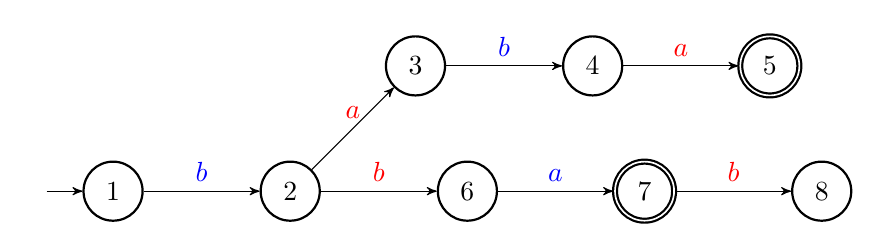
\begin{tikzpicture}
        \tikzset{
          ->,
          >=stealth',
          node distance=2.25cm,
          every state/.style={
            thick,
            inner sep = 0pt,
            minimum size = 0.75cm,
          },
          initial text=$ $,
        }
        \node[state, initial] (q1) {\(1\)};
        \node[state, right of=q1] (q2) {\(2\)};
        \node[state, above right of=q2] (q3) {\(3\)};
        \node[state, right of=q3] (q4) {\(4\)};
        \node[state, accepting, right of=q4] (q5) {\(5\)};
        \node[state, right of=q2] (q6) {\(6\)};
        \node[state, accepting, right of=q6] (q7) {\(7\)};
        \node[state, right of=q7] (q8) {\(8\)};

        \draw
          (q1) edge[above] node[blue]{\(b\)} (q2)
          (q2) edge[above] node[red]{\(a\)} (q3)
          (q3) edge[above] node[blue]{\(b\)} (q4)
          (q4) edge[above] node[red]{\(a\)} (q5)
          (q2) edge[above] node[red]{\(b\)} (q6)
          (q6) edge[above] node[blue]{\(a\)} (q7)
          (q7) edge[above] node[red]{\(b\)} (q8);
      \end{tikzpicture}

      \pause[]

      \vphantom{}

      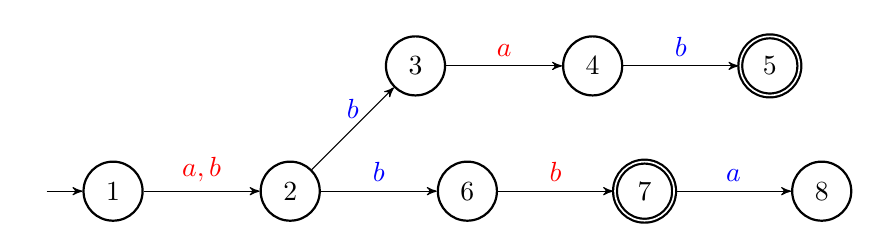
\begin{tikzpicture}
        \tikzset{
          ->,
          >=stealth',
          node distance=2.25cm,
          every state/.style={
            thick,
            inner sep = 0pt,
            minimum size = 0.75cm,
          },
          initial text=$ $,
        }
        \node[state, initial] (q1) {\(1\)};
        \node[state, right of=q1] (q2) {\(2\)};
        \node[state, above right of=q2] (q3) {\(3\)};
        \node[state, right of=q3] (q4) {\(4\)};
        \node[state, accepting, right of=q4] (q5) {\(5\)};
        \node[state, right of=q2] (q6) {\(6\)};
        \node[state, accepting, right of=q6] (q7) {\(7\)};
        \node[state, right of=q7] (q8) {\(8\)};

        \draw
          (q1) edge[above] node[red]{\(a, b\)} (q2)
          (q2) edge[above] node[blue]{\(b\)} (q3)
          (q3) edge[above] node[red]{\(a\)} (q4)
          (q4) edge[above] node[blue]{\(b\)} (q5)
          (q2) edge[above] node[blue]{\(b\)} (q6)
          (q6) edge[above] node[red]{\(b\)} (q7)
          (q7) edge[above] node[blue]{\(a\)} (q8);
      \end{tikzpicture}
    }
    \only<3-4> {
      \begin{tikzpicture}
        \tikzset{
          ->,
          >=stealth',
          node distance=2.25cm,
          every state/.style={
            thick,
            inner sep = 0pt,
            minimum size = 0.75cm,
          },
          initial text=$ $,
        }
        \node[state, initial] (q1) {\(1\)};
        \node[state, right of=q1] (q2b) {\(2_b\)};
        \node[state, left of=q3] (q2a) {\(2_a\)};
        \node[state, above right of=q2b] (q3) {\(3\)};
        \node[state, right of=q3] (q4) {\(4\)};
        \node[state, accepting, right of=q4] (q5) {\(5\)};
        \node[state, right of=q2] (q6) {\(6\)};
        \node[state, accepting, right of=q6] (q7) {\(7\)};
        \node[state, right of=q7] (q8) {\(8\)};

        \draw
          (q1) edge[above] node[blue]{\(b\)} (q2a)
          (q1) edge[above] node[blue]{\(b\)} (q2b)
          (q2a) edge[above] node[red]{\(a\)} (q3)
          (q3) edge[above] node[blue]{\(b\)} (q4)
          (q4) edge[above] node[red]{\(a\)} (q5)
          (q2b) edge[above] node[red]{\(b\)} (q6)
          (q6) edge[above] node[blue]{\(a\)} (q7)
          (q7) edge[above] node[red]{\(b\)} (q8);
      \end{tikzpicture}

      \pause[4]

      \vphantom{}

      \begin{tikzpicture}
        \tikzset{
          ->,
          >=stealth',
          node distance=2.25cm,
          every state/.style={
            thick,
            inner sep = 0pt,
            minimum size = 0.75cm,
          },
          initial text=$ $,
        }
        \node[state, initial] (q1) {\(1\)};
        \node[state, right of=q1] (q2b) {\(2_b\)};
        \node[state, left of=q3] (q2a) {\(2_a\)};
        \node[state, above right of=q2b] (q3) {\(3\)};
        \node[state, right of=q3] (q4) {\(4\)};
        \node[state, accepting, right of=q4] (q5) {\(5\)};
        \node[state, right of=q2] (q6) {\(6\)};
        \node[state, accepting, right of=q6] (q7) {\(7\)};
        \node[state, right of=q7] (q8) {\(8\)};

        \draw
          (q1) edge[above] node[red]{\(a\)} (q2a)
          (q1) edge[above] node[red]{\(b\)} (q2b)
          (q2a) edge[above] node[blue]{\(b\)} (q3)
          (q3) edge[above] node[red]{\(a\)} (q4)
          (q4) edge[above] node[blue]{\(b\)} (q5)
          (q2b) edge[above] node[blue]{\(b\)} (q6)
          (q6) edge[above] node[red]{\(b\)} (q7)
          (q7) edge[above] node[blue]{\(a\)} (q8);
      \end{tikzpicture}
    }
  \end{example}
\end{frame}

\begin{frame}{\myframetitle}
  \begin{block}{Automate quelconque}
    Si on ajoute les cycles, on devra alors supposer que tous n\oe{}uds
    intermédiaire se trouve dans le cas du n\oe{}ud \(2\), on devra donc le
    dupliquer.
  \end{block}
\end{frame}

\begin{frame}{\myframetitle}
  \begin{example}
    \centering
    \only<1-2> {
      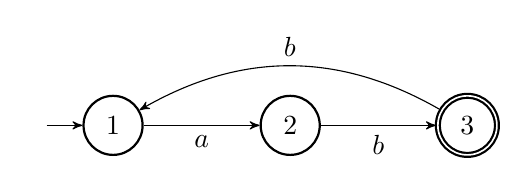
\begin{tikzpicture}
        \tikzset{
          ->,
          >=stealth',
          node distance=2.25cm,
          every state/.style={
            thick,
            inner sep = 0pt,
            minimum size = 0.75cm,
          },
          initial text=$ $,
        }
        \node[state, initial] (1) {\(1\)};
        \node[state, right of=1] (2) {\(2\)};
        \node[state, accepting, right of=2] (3) {\(3\)};
        \draw
          (1) edge[below] node{\(a\)} (2)
          (2) edge[below] node{\(b\)} (3)
          (3) edge[bend right, above] node{\(b\)} (1);
      \end{tikzpicture}
    }
    \only<2> {
      \begin{tikzpicture}
        \tikzset{
          ->,
          >=stealth',
          node distance=2.25cm,
          every state/.style={
            thick,
            inner sep = 0pt,
            minimum size = 0.75cm,
          },
          initial text=$ $,
        }
        \node[state, initial] (1) {\(1\)};
        \node[state, above of=3] (1a) {\(1_a\)};
        \node[state, right of=1] (2b) {\(2_b\)};
        \node[state, above of=2b] (2) {\(2\)};
        \node[state, accepting, right of=2b] (3) {\(3\)};
        \node[state, accepting, above of=1] (3b) {\(3_b\)};
        \draw
          (1) edge[below] node{\(b\)} (2b)
          (2b) edge[below] node{\(a\)} (3)
          (3) edge[right] node{\(a\)} (1a)
          (1a) edge[above] node{\(b\)} (2)
          (2) edge[above] node{\(b\)} (3b)
          (3b) edge[left] node{\(b\)} (1);
      \end{tikzpicture}
    }
  \end{example}
\end{frame}

\begin{frame}{\myframetitle}
  \begin{block}{Compléxité en état de notre algorithme}
    Dans le pire cas, notre algorithme dupliquera tous les états de
    l'automate. 

    \pause[]
    \vphantom{}

    Sachant que chaque état peut être dupliqué étant de voir qu'il y a de
    symbole de l'alphabet plus un. 

    \pause[]
    \vphantom{}

    Alors, la complexité dans le pire cas de notre algorithme est \(n(\lvert
    \Sigma \rvert + 1)\).
  \end{block}
\end{frame}

\section{Conclusion}

Durant cet article, nous avons défini deux transformations particulières
de langages réguliers~: le trognon d’un langage et le langage permuté. Pour
chacune d’elles, nous avons conçu un algorithme capable de construire, à
partir d’un automate non déterministe initial, un nouvel automate
reconnaissant le langage transformé.

\vphantom{}

Nous avons également fourni une preuve de correction pour chaque algorithme,
montrant que les automates produits reconnaissent exactement les langages
visés. Enfin, nous avons analysé la complexité en nombre d’états dans le pire
des cas.

\vphantom{}

Des perspectives intéressantes s’ouvrent à la suite de ce travail. En
particulier, affiner les bornes de complexité.


\printbibliography

\end{document}
